\documentclass[preprint]{IEIE} % for review
\usepackage{graphicx}
% 참고문헌 항목 간 간격 최소화 (분량 조절)
\makeatletter
\renewcommand\@openbib@code{\setlength{\itemsep}{0pt}\setlength{\parsep}{0pt}}
\makeatother
\title{범용 마이크로컨트롤러에서 스파이킹 신경망의\\이벤트 구동 이득 회수: 비트 동일 무곱셈 희소 커널의\\설계 원리와 STM32F746 실측}
\author{차주형 \\ 과학기술연합대학원대학교(UST) \\ e-mail : chacha@ust.ac.kr}
\engtitle{Reclaiming the Event-Driven Advantage of Spiking Neural Networks\\on a Commodity Microcontroller: Design Principles and Measurements\\of a Bit-Exact, Multiplication-Free Sparse Kernel}
\engauthor{JooHyoung Cha \\ University of Science and Technology (UST)}
\abstract{
The efficiency narrative of spiking neural networks (SNNs) rests on an algebraic fact: activations are binary events, so inference needs additions, not multiplications, and only where spikes occur. Neuromorphic processors realize this in silicon, yet when SNNs are deployed on commodity microcontrollers through standard TinyML stacks, the same networks are lowered to dense tensor kernels that multiply mostly zeros---the advantage is forfeited at the kernel boundary, not in the model. We argue that the event-driven advantage is a property of the arithmetic, not of the hardware, and can therefore be reclaimed in software, exactly. We formulate the reclamation as three design principles---(1) materialize spike \emph{positions}, not activation values, eliminating im2col entirely; (2) assign the irregular (event) axis to indexing and the regular (channel) axis to contiguous streaming, via a transposed weight layout with register-blocked accumulation; (3) keep the integer epilogue invariant, turning bit-exactness into a verifiable contract---and instantiate them as a multiplication-free convolution kernel inside TensorFlow Lite for Microcontrollers with CMSIS-NN. A measurement-first diagnosis on an STM32F746 (Cortex-M7, 200MHz) precedes the design: cycle-accurate ablations falsify the presumed instruction-fetch bottleneck (flash-ART enablement and ITCM code placement each shift latency by at most 0.12\%) and locate the cost in data movement for zero operands. On CIFAR-10 rate-coded inference ($T{=}30$), the kernel reduces per-image latency from a reproduced 2,328.5ms baseline to 380.6ms (6.12$\times$) and accelerates the 4.1\%-density hidden convolution 13.0$\times$ over the equally-placed dense kernel, with output spikes bit-identical across all six build variants; the TFLM integration costs 2.1\% relative to a runtime-free invocation of the same optimized path. A first-order cost model fitted to the measurements places the sparse--dense break-even near 89\% activation density, implying the sparse regime covers virtually the entire operating range of SNNs.
\par\vspace{0.5\baselineskip}\noindent
\textbf{Keywords} --- Spiking Neural Network, Event-Driven Inference, Spike Sparsity, Multiplication-Free Kernel, TinyML, CMSIS-NN, Cortex-M7

}

\begin{document}
\maketitle
\makeabstract

\section{서론}\label{sec:intro}

스파이킹 신경망(Spiking Neural Network, SNN)의 효율성 서사는 하나의
대수적 사실에 기초한다. 뉴런 간에 오가는 것이 실수 활성값이 아니라
이진 스파이크이므로, 추론의 기본 연산은 곱셈-누산(MAC)이 아니라
\emph{발화한 곳의 가중치를 더하는 것}으로 충분하다는 사실이다
\cite{maass1997networks,roy2019towards}. 덧셈은 곱셈-누산보다 수 배
싸고\cite{horowitz2014computing}, 발화는 희소하므로 더할 일
자체가 드물다. 이 두 성질 --- 무곱셈성과 이벤트 희소성 --- 이 SNN이
약속하는 효율의 원천이며, Loihi나 TrueNorth 같은 뉴로모픽
프로세서는 이 약속을 실리콘 수준에서
구현한다\cite{davies2018loihi,merolla2014truenorth}.

문제는 이 약속이 \emph{배포 경로에서 소멸}한다는 데 있다. 이미
대규모로 보급된 범용 마이크로컨트롤러(MCU) 위에 SNN을 올리는 현실적
경로는 표준 TinyML 스택 --- TensorFlow Lite for
Microcontrollers(TFLM)\cite{david2021tflm}와
CMSIS-NN\cite{lai2018cmsisnn} --- 이고, 이 스택의 커널은 조밀(dense)
텐서 산술을 전제한다. 이진 스파이크는 int16 텐서로 실체화되어 dense
MAC 루프에 공급되고, 프로세서는 대부분이 0인 피연산자를 성실하게
읽어 와서 곱한다. 즉 모델은 이벤트를 말하는데 커널은 텐서를
계산한다. 저자의 선행 연구\cite{cha2026fusion}가 그 전형이다:
Conv-AvgPool-LIF 퓨전 연산자를 TFLM에 통합하여 표준 경로 대비 4.0배를
얻었지만, 커널 자체는 dense SMLALD 누산이었고 도달 처리량은 칩
이론 피크의 약 18\%에 머물렀다. 그 사이 실측된 은닉층 발화율은
4.1\% --- 지배 레이어 연산의 약 96\%가 0과의 곱셈이었다.

본 논문의 논제는 다음과 같다. \textbf{SNN의 이벤트 구동 이득은
하드웨어의 성질이 아니라 산술의 성질이므로, 하드웨어를 바꾸지 않고
커널 수준에서, 그것도 비트 단위로 동일하게 회수할 수 있다.} 입력이
$\{0, S\}$ 이진이면 내적은 다음과 같이 붕괴한다:
$\sum_k w_k x_k = S\cdot\sum_{x_k\neq0}w_k$. 이 항등식은 정수 산술의
결합$\cdot$교환법칙 위에서 성립하므로, 이를 구현한 커널은 근사
가속기가 아니라 \emph{의미를 보존하는 프로그램 변환}이다. 회수를
실제 성능으로 연결하기 위해 본 논문은 세 가지 설계 원리를 제시한다:
(P1) 활성 \emph{값}이 아니라 발화 \emph{위치}를 실체화하라 ---
im2col이 통째로 사라진다; (P2) 불규칙한 이벤트 축은 인덱스로,
규칙적인 채널 축은 연속 스트림으로 배정하라 --- 가중치 전치와
레지스터 블로킹이 그 귀결이다; (P3) 정수 에필로그를 불변으로 지켜라
--- 비트 동일성이 검증 가능한 계약이 된다.

본 논문의 두 번째 논제는 방법론적이다. \textbf{커널을 다시 쓰기
전에, 병목의 위치는 대상 워크로드 위의 절제(ablation) 실측으로
확정되어야 한다.} 사전 하드웨어 조사가 유망하게 지목한 두 가지 명령
페치 최적화 --- 플래시 가속기(ART) 활성화와 핫 커널의 ITCM-RAM 배치
--- 는 마이크로벤치마크에서는 각각 1.4배$\cdot$2.5배급 효과였으나,
실제 추론 워크로드에서는 $\le$0.12\%의 변화에 그친 실질 무효과였다.
우리는 그 원인(부팅 주소와 실행 주소의 불일치, 핫 루프와 캐시
용량의 관계)을 규명하고, 병목이 ``0을 곱하기 위한 데이터
이동''임을 사이클 수준 회계로 특정한 뒤에야 커널을 재설계했다.
이 진단 과정과 부정적 결과를 본문에 그대로 보고한다.

기여는 다음과 같이 요약된다.
\begin{itemize}
\item \textbf{개념화}: MCU 위 SNN 추론에서 이벤트 구동 이득이
  소멸하는 지점을 커널 경계로 특정하고, 그 회수를 세 가지 설계
  원리(P1--P3)와 의미 보존 계약으로 정식화한다(IV장).
\item \textbf{진단 방법론}: 조건을 레지스터로 증명하고 결과를 출력
  체크섬으로 불변식화한 사이클 정밀 절제 실측으로, 통념적 병목
  가설 2종을 반증하고 데이터 이동 병목을 확정한다(III장).
\item \textbf{구현과 실측}: 제안 커널은 TFLM 커스텀 연산자 프레임과
  CMSIS-NN 지원 함수 위에 그대로 얹히며, STM32F746 실측에서 종단
  $6.12$배($2{,}328.5\rightarrow380.6$ms/이미지), 발화율 4.1\%
  레이어 13.0배(동일 배치 dense 대비)를 여섯 빌드 변형의 출력 비트
  일치와 함께 달성한다(V장).
  런타임 오버헤드는 2.1\%에 머문다.
\item \textbf{일반화}: 실측에 적합시킨 1차 비용 모델로 희소-조밀
  손익분기 밀도를 약 89\%로 추정한다 --- SNN의 통상 동작 영역
  전체가 희소 커널의 우세 구간에 들어온다(VI장).
\end{itemize}

이후 구성은 다음과 같다. II장은 관련 연구 속에서 본 연구의 위치를
정한다. III장은 대상 시스템과 진단 방법론, 그리고 병목의 확정을
다룬다. IV장은 설계 원리와 그 구현$\cdot$비용 모델을, V장은 연구
질문 네 개에 대한 실측 답을 제시한다. VI장은 일반화와 한계를
논의하고 VII장에서 결론을 맺는다.


\section{배경 및 관련 연구}\label{sec:related}

\subsection{SNN 효율 논거의 실체}\label{sec:premise}

SNN 문헌의 효율 논거는 통상 연산 단가표에서 출발한다. 45nm 32비트
부동소수점 기준으로 곱셈-누산은 4.6pJ, 덧셈은 0.9pJ라는
단가표\cite{horowitz2014computing}가 그것으로, 활성값이 이진인 SNN은
곱셈을 덧셈으로 대체하므로 발화율 $R$과 타임스텝 $T$가 작으면
$E_{AC}\!\cdot\!T\!\cdot\!R < E_{MAC}$로 이득이라는 형태의 손익
조건이 도출된다\cite{yao2023spikedriven}. 그러나 이 전제를 상용
프로세서로 옮기면 두 가지 정정이 필요하다. 첫째, 단가표는 데이터패스
\emph{회로}의 에너지에 관한 것이다. 파이프라인화된 MCU에서 곱셈은
이미 단일 사이클 명령(예: Cortex-M7의 SMLAD)이므로, ``곱셈을
덧셈으로 바꾸는 것'' 자체는 시간으로는 거의 아무것도 벌지 못한다.
둘째, 문헌의 정밀 분석들이 수렴하는 결론은 이득의 원천이 연산
치환이 아니라 \emph{희소성}이라는 것이다. Dampfhoffer 등은 디지털
하드웨어 모델에서 VGG16급 SNN의 시냅스 연산이 전체 에너지의 약
1\%에 불과하며 지배 항은 메모리 접근임을 보이고, SNN이 우세해지는
조건을 스파이크
희소성으로 귀속시킨다\cite{dampfhoffer2023snns}. Davidson과
Furber는 뉴런당 약 1.7 스파이크를 손익분기로 제시하며 rate 코딩
SNN의 이득에 회의적이고\cite{davidson2021comparison}, 반대편에는
6--8배 이득을 추정하는 분석도 있다\cite{lemaire2022analytical}.
추정이 가정에 따라 무이득에서 8배까지 갈린다는 사실 자체가, 고정된
상용 타깃 위의 \emph{실측}이 필요하다는 본 논문의 방법론적 입장을
뒷받침한다. 본 논문의 실측은 이 결론의 시간 영역 대응물을
제공한다: 인오더 MCU에서는 메모리 정지 사이클이 곧 시간 비용이므로
같은 구조가 지연에서도 나타나리라 기대할 수 있고, 실제로 병목은
0-피연산자의 메모리 이동으로 실측되었으며(III장), 그 트래픽을
제거한 커널이 단독 5.7배 --- 종단 구성 기준 6.12배 --- 를 냈다(V장).

\subsection{전용 실리콘의 회수}\label{sec:silicon}

이벤트 구동 이득을 하드웨어로 회수하는 길은 뉴로모픽 프로세서가
대표한다. TrueNorth\cite{merolla2014truenorth},
SpiNNaker\cite{furber2014spinnaker},
Loihi\cite{davies2018loihi}와 그 2세대\cite{orchard2021loihi2}는
스파이크가 있을 때만 연산이 일어나는 실행 모델을
실리콘$\cdot$시스템 수준에서 구현했고,
최근의 Speck은 완전 비동기 SoC에서 소비 전력이 입력 이벤트양에
비례함을 보였다\cite{yao2024speck}. 본 연구는 이 노선의 대체가
아니라 보완이다: 전용 실리콘 없이, 이미 보급된 상용 MCU에서, 같은
비례성의 \emph{산술적} 몫이 얼마나 회수되는지를 묻는다.

\subsection{희소성 활용 추론 시스템}\label{sec:sparse-sys}

DNN 일반에서 0-피연산자를 건너뛰려는 시도는 가속기 설계에서
시작되었다. Cnvlutin은 0 활성값의 곱셈을 동적으로
생략했고\cite{albericio2016cnvlutin}, EIE는 압축 표현 위에서
FC 층의 제로 스킵을\cite{han2016eie}, SCNN은 비영 쌍만 곱셈기에
전달하는 데이터플로를\cite{parashar2017scnn} 구현했다 --- 모두 전용
실리콘을 전제한다. 범용 CPU에서는 정적 가중치 희소성을 CSR류
형식으로 소비하는 직접 희소 합성곱(3--7배)\cite{park2017faster}과,
ReLU 활성 희소성을 학습으로 유도해 소비하는
커널\cite{kurtz2020inducing}이
서버급(x86, 광폭 벡터, GB급 메모리)에서 이득을 보였다.
공간 희소 데이터 쪽에서는 활성 좌표 집합에 합성곱을 제한하는
submanifold 방식\cite{graham2018submanifold}과 이벤트 카메라 입력의
비동기 희소 합성곱\cite{messikommer2020event}이 있으나, 전자는 GPU
라이브러리이고 후자의 절감은 주로 연산량(FLOP) 수준에서 보고된다.
우리가 확인한 범위에서 이 계열 중 MCU급(Cortex-M, RAM $<$1MB)
장치를 다룬 것은 없다. 또한 SNN의 이진 활성은 이 계열과 결이 다른
이점을 준다: 값이 $\{0,S\}$뿐이므로 희소 소비가 값 적재 없는
\emph{위치 전용} gather가 되고(IV장 원리 1), im2col류의 값
실체화\cite{chellapilla2006high} 자체가 원리적으로 불필요해진다.

\subsection{MCU 위의 SNN과 본 연구의 위치}\label{sec:positioning}

SNN 소프트웨어 스택은 학습 쪽으로
성숙했다\cite{eshraghian2023training,fang2023spikingjelly,pehle2021norse}.
그러나 배포 경로는 뉴로모픽 백엔드를 지향하거나 이식 표준의
단계\cite{pedersen2024nir}에 있고, MCU 급 상용 하드웨어를 향한
실측 연구는 이제 축적되는 중이다. Barchi 등은 STM32 계열에서 순환
SNN의 근접 센서 추론을 보였고\cite{barchi2021shm}, 후속 연구에서는
발화 활동 자체를 모델 수준에서 조율해 지연과 에너지를
낮췄다\cite{barchi2024tuning} --- 스파이크
수를 \emph{줄이는} 접근으로, 스파이크당 비용을 줄이는 본 연구와
직교한다. Jurzec 등은 snnTorch 모델을 자체 C 런타임으로 내려 Cortex-M7
보드에 올렸으나 희소성은 지속 비활성 뉴런의 오프라인 프루닝으로
쓰였고 속도 수치는 데스크톱 기준이다\cite{jurzec2025compression}.
개념적으로 가장 가까운 것은 Liao 등의 뇌-기계 인터페이스
디코더로, 병렬 RISC-V(GAP9)에서 발화한 뉴런의 가중치 열만 DMA로
가져오는 ``sparse copy''를 구현했다\cite{liao2024snndecoder} ---
발화로 가중치 트래픽을 게이팅한다는 착상을 공유하지만, 대상이
FC/순환 디코더라 수용 영역 인덱싱$\cdot$im2col 문제가 없고, 전용
런타임이며, 정확성은 근사 수준(``무시할 손실'')으로 보고된다.
SpikeStream은 희소 SNN 추론을 위해 RISC-V ISA에 간접 스트림
확장을 추가해 4.4배를 얻었는데\cite{manoni2025spikestream}, 이는
역으로 상용 ISA 그대로는 어렵다는 방증으로 읽을 수 있다 --- 본
연구는 그 간접 스트리밍을 전치 레이아웃과 레지스터 블로킹의 순수
소프트웨어로 대신한다(IV장 원리 2).

표~\ref{tab:positioning}이 위치를 요약한다. 우리가 조사한 범위에서,
\textbf{상용 Cortex-M급 MCU에서, 표준 TinyML 런타임 안에서, 합성곱
SNN의 발화 희소성을 런타임에 소비하며 조밀 경로와의 비트 동일성을
보증한 실측 보고는 본 연구가 처음이다}.

\begin{table*}[t]
\centering
\caption{희소성 활용 추론 연구들 속에서의 위치. ($\circ$: 해당,
$\triangle$: 부분적, $\times$: 비해당, --: 무관)}
\label{tab:positioning}
\footnotesize
\setlength{\tabcolsep}{5pt}
\begin{tabular}{l l l l c c}
\hline
연구 & 실행 기반 & 희소성 활용 방식 & 합성곱 & 표준 런타임 & 비트 동일 보증 \\
\hline
Speck\cite{yao2024speck} & 비동기 뉴로모픽 SoC & 실리콘 이벤트 구동 & $\circ$ & -- & -- \\
SCNN\cite{parashar2017scnn} & 전용 가속기(ASIC) & 비영 쌍 전달 하드웨어 & $\circ$ & -- & -- \\
Kurtz 등\cite{kurtz2020inducing} & x86 서버(AVX) & 유도 ReLU 희소성, SW & $\circ$ & $\times$ & $\triangle$ \\
SpikeStream\cite{manoni2025spikestream} & RISC-V 클러스터 & 간접 스트림 ISA 확장 & $\circ$ & $\times$ & $\times$ \\
Liao 등\cite{liao2024snndecoder} & GAP9 병렬 RISC-V & 발화 열 DMA 게이팅 & $\times$(FC/순환) & $\times$ & $\times$ \\
Barchi 등\cite{barchi2024tuning} & STM32(Cortex-M) & 모델 수준 발화 감소 & $\times$(순환) & $\times$ & $\times$ \\
Jurzec 등\cite{jurzec2025compression} & STM32H747(M7) & 오프라인 프루닝 & $\triangle$ & $\times$ & $\times$ \\
\textbf{본 연구} & \textbf{STM32F746(M7)} & \textbf{런타임 이벤트 게이팅, SW}
& $\circ$(수용 영역 인덱스) & $\circ$(TFLM$+$CMSIS-NN) & $\circ$(체크섬) \\
\hline
\end{tabular}
\begin{flushleft}
\footnotesize 주: ``비트 동일 보증''은 조밀 정수 경로와의 비트 단위
등가를 기계 검증하는지의 여부다. Kurtz 등의 커널은 수학적으로
정확하나 대상이 부동소수점 서버 추론이라 본 표의 관점(정수 경로
등가 검증)과는 구별된다.
\end{flushleft}
\end{table*}

\subsection{본 파이프라인의 발화 밀도}\label{sec:sparsity}

희소 커널의 이득은 전적으로 발화 밀도에 걸려 있으므로, 대상
파이프라인의 밀도를 먼저 실측해 둔다. 선행
연구\cite{cha2026fusion}는 희소성 활용을 향후 과제로 남기며 발화율을
보고하지 않았기에, 저자는 같은 모델$\cdot$같은 정수 파이프라인의
호스트 구현으로 CIFAR-10 테스트셋 10{,}000장$\times$30스텝을 전수
측정했다: 비영 활성 비율은 입력 스파이크 47.7\%, 첫 합성곱
출력(LIF1) 4.1\%, 둘째 출력(LIF2) 3.4\%다. 은닉층은 문헌의 통상
관측대로 수 퍼센트대이나 입력층은 rate 코딩 탓에 예외적으로
조밀하다 --- rate 코딩이 시간 코딩 대비 약 7배 많은 스파이크를
쓴다는 비교 분석\cite{guo2021neural}과 정합하는 값이다. 이 비대칭은
IV장의 비용 모델이 예측할 레이어 간 이득 격차의 원인이며, 스파이크
수 자체를 줄이는 학습 측 기법\cite{sorbaro2020optimizing}이 본
커널과 직교로 결합될 수 있는 이유이기도 하다.


\section{문제 설정과 진단}\label{sec:problem}

\subsection{대상 시스템과 성능 간극}\label{sec:target}

대상은 선행 연구\cite{cha2026fusion}가 구축한 SNN 추론
파이프라인이다. CIFAR-10\cite{krizhevsky2009cifar} 입력을 rate
coding으로 타임스텝마다 이진 스파이크($0$ 또는 $32{,}767$, Q15의
1.0)로 인코딩하고, [Conv $5{\times}5$ + AvgPool + LIF] 두 단과 FC,
출력 LIF를 $T{=}30$회 반복한다. LIF 뉴런은 Q15 고정소수점
감쇠($\beta{=}29{,}491\approx0.9$), 임계값 $32{,}767$, 감산 리셋으로
동작하며, snnTorch\cite{eshraghian2023training}와
Brevitas\cite{brevitas2023}의 QAT 학습
결과\cite{jacob2018quantization}를 정수 전용으로 변환한 것이다. 배포
시 각 Conv+AvgPool 쌍은 $6{\times}6$ stride-2 커널로 대수 퓨전되고
(가중치는 int8 4개의 합인 int16, $|w|\le508$), TFLM 커스텀 연산자가
CMSIS-NN 지원 함수와 함께 이를 실행한다. 표~\ref{tab:model}가 퓨전
후 형상이다. 두 번째 합성곱(CPL2)이 타임스텝당 5.64M MAC의
83.6\%를 차지한다.

\begin{table}[htbp]
\centering
\caption{퓨전 후 레이어 구성과 타임스텝당 MAC.}
\label{tab:model}
\footnotesize
\setlength{\tabcolsep}{3.5pt}
\begin{tabular}{l l l r r}
\hline
레이어 & 입력 & 출력 & $r$(열 길이) & MAC/스텝 \\
\hline
CPL1 & $32{\times}32{\times}3$ & $16{\times}16{\times}32$ & 108 & 884,736 \\
CPL2 & $16{\times}16{\times}32$ & $8{\times}8{\times}64$ & 1,152 & 4,718,592 \\
FC & 4,096 & 10 & -- & 40,960 \\
\hline
\multicolumn{4}{l}{합계 (이미지당 $\times 30$)} & 5,644,288 \\
\hline
\end{tabular}
\begin{flushleft}
\footnotesize 주: $r = k_h k_w C_i$는 합성곱을 행렬곱으로 볼 때의
내적 길이. CPL $=$ Conv+AvgPool+LIF 퓨전 연산자.
\end{flushleft}
\end{table}

선행 실측은 이미지당 $2{,}407.0$ms였다\cite{cha2026fusion}. 이는
비퓨전 표준 경로의 4.0배지만, 유효 처리량으로는 약 70MMAC/s ---
이 칩(Cortex-M7, SMLAD 사이클당 2 MAC, 200MHz에서
400MMAC/s)의 약 18\%다. 남은 5.7배의 간극이 본
연구의 출발점이며, 간극의 원인 후보는 둘이다: 명령을 공급하지
못해서인가(페치 병목), 데이터를 공급하지 못해서인가(로드 병목).
그리고 후자라면, II장의 관찰이 가리키듯 그 데이터의 대부분은 곱해
봐야 0인 피연산자다.

\subsection{진단 방법론: 성능 주장을 인과 주장으로}\label{sec:method}

``최적화 X가 성능을 개선했다''는 주장은 인과 주장이고, 인과 주장이
성립하려면 세 요소가 필요하다. (i) \textbf{조건의 증명}: 라벨이
아니라 실리콘이 답한 상태로 측정 조건을 기록해야 한다. 우리는 매
측정에 \texttt{FLASH\_ACR}$\cdot$\texttt{SCB\_CCR} 레지스터 값과
ITCM 적재 바이트 수를 동봉해, 각 변형이 주장하는 조건이 실제로
성립했음을 증명한다. (ii) \textbf{결과의 불변식}: 빨라진 코드가
같은 것을 계산하는지 기계적으로 판정해야 한다. 우리는 출력
스파이크의 비트 체크섬(V장)을 모든 변형에 요구한다. (iii)
\textbf{단일 요인 절제}: 최적화를 하나씩 누적한 빌드
변형(A0--A4)을 같은 하네스에서 측정한다.

하네스는 이 세 요소를 위해 설계되었다: 입력은 플래시에 고정된
CIFAR-10 테스트 이미지 8장(SD카드$\cdot$JPEG$\cdot$표시 경로 배제),
인코딩 난수는 시드 고정 xorshift32, 시간은 DWT 사이클
카운터(1사이클 해상도), 워밍업 1장은 제외한다. 하네스 자신도 검증
대상이다: 독립 검토에서 타임베이스 인터럽트 침투(약 0.1\%
노이즈)$\cdot$누산기 자릿수$\cdot$결과 회수 주소 오류 3건이 발견되어
수정 후 절제 변형(A0--A4) 전량을 재측정했다. 선행 연구의 $2{,}407.0$ms는 1ms 해상도
시계$\cdot$표시 루프 포함$\cdot$다른 입력 집합의 수치이므로, 본
하네스로 동일 코드 경로를 재현한 $2{,}328.5$ms(차이 3.3\%)를
기준선(A0)으로 삼고 이후 모든 배속을 하네스 내부 상대 비교로만
계산한다.

\subsection{페치 가설의 반증}\label{sec:falsify}

사전 하드웨어 조사는 페치 병목을 강하게 시사했었다. 이 보드는 옵션
바이트에 의해 플래시의 ITCM 별칭 주소에서 부팅하는데 그 경로의
캐시인 ART 가속기가 꺼져 있었고(\texttt{FLASH\_ACR}$=$0x006),
마이크로벤치마크에서 ART 활성화는 해당 경로를 1.4배 이상, 코드의
ITCM-RAM 이전은 최대 2.5배 가속했다. 그러나 실제 추론 워크로드의
절제 실측(V장 표~\ref{tab:ablation})에서 두 최적화는 \textbf{모두
실질 무효과}였다($\le$0.12\%; A2의 소폭 퇴행은 ITCM 왕복 베니어
오버헤드로 추정된다): ART 활성화(A1)
$2{,}328.5\rightarrow2{,}328.9$ms, 핫 커널 $4{,}392$B의 ITCM
배치(A2) $\rightarrow2{,}331.2$ms.

반증의 기제는 두 가지다. 첫째, \textbf{부팅 주소와 실행 주소는
다르다}. 리셋 벡터는 ITCM 별칭에서 읽히지만 링커는 코드를 AXIM
주소에 배치했으므로, 이후 모든 페치는 AXIM 경로로 나가고 그 경로는
이미 L1 I-캐시가 담당한다. ART는 ITCM 경로 전용이라 개입할 자리가
없다. 둘째, \textbf{핫 명령 집합이 캐시보다 훨씬 작다}. 실행 시간의
대부분을 차지하는 내적 루프는 수백 바이트로 4KB I-캐시에 상주한다.
마이크로벤치마크의 ``큰 커널'' 조건은 6KB 코드를 균일 순회하는 합성
지역성이었고, 실제 워크로드의 지역성과 달랐던 것이다. 이 결과는
마이크로벤치마크 기반 병목 추정의 위험을 보여주는 부정적 증거로서
기록한다.

\subsection{데이터 이동 병목의 확정}\label{sec:datamove}

페치가 아니면 데이터다. dense 커널의 CPL2는 출력 픽셀 2개를 계산할
때마다 퓨전 가중치 전체($147{,}456$B)를 다시 읽는다. 가중치
트래픽만 타임스텝당 약 4.7MB, 이미지당 141.6MB로, 4KB
D-캐시를 상시 축출하는 스트림이다. 실제로 데이터의 \emph{위치}만
바꾼 절제 변형(A3: 가중치$\cdot$LIF 상태$\cdot$스크래치의
DTCM/SRAM 재배치)은 7\%를 얻는 데 그쳤다 --- 144KB 스트림이 4KB
캐시를 축출하는 구조가 그대로인 한 라인필 횟수는 변하지 않으므로,
배치 개선의 여지가 이 수준에 그친다는 방증이다.

총량을 줄이는 유일한 지렛대는 ``곱해 봐야 0인 피연산자를 아예 읽지
않는 것''이고, II장에서 본 것처럼 CPL2 입력의 약 96\%가 그런
피연산자다. 문제는 이로써 명확한 형태를 갖춘다: \emph{희소성을
커널이 소비할 수 있는 형태로 바꾸되, 정수 의미를 비트 단위로
보존하라}. 다음 장이 그 설계다.


\section{설계: 이벤트 집합 위의 합성곱}\label{sec:design}

이 장은 제안 커널 --- 이하 \emph{이벤트 커널}이라 부른다(제목의
무곱셈 희소 커널과 동일한 대상이다) --- 을 구현 절차가 아니라
원리의 체계로 서술한다.
출발점은 회수하려는 성질을 정확히 명제로 만드는 것이고(4.1절),
본체는 그 명제를 실제 성능으로 바꾸는 세 가지 설계
원리다(4.2--4.4절). 구현은 원리의 귀결로서 간략히
정리하고(4.5절), 마지막으로 이득의 구조를 1차 비용 모델로
추상화한다(4.6절). 그림~\ref{fig:concept}이 전체 대비를 요약한다.

\begin{figure}[htbp]
\centering
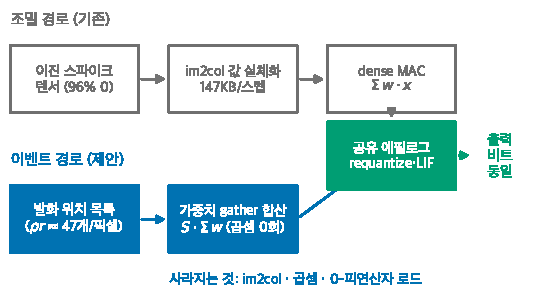
\includegraphics[width=0.98\linewidth]{figures/fig_concept.pdf}
\caption{조밀 경로(위)와 이벤트 경로(아래). 이진 활성에서는 값
실체화(im2col)와 곱셈이 원리적으로 불필요하다. 두 경로는 동일한
정수 에필로그를 공유하므로 출력이 비트 단위로 같다.}
\label{fig:concept}
\end{figure}

\subsection{대수적 기초와 의미 보존 계약}\label{sec:contract}

이 파이프라인의 모든 합성곱 입력은 이진이다: 첫 단은 인코더
출력 $\{0, 32{,}767\}$, 둘째 단은 LIF 스파이크 $\{0, S_1\}$이며,
제로 패딩은 비발화와 구별되지 않는다. 입력이 $\{0,S\}$이면 내적
길이 $r$의 곱셈-누산은 다음으로 붕괴한다:
\begin{equation}
\sum_{k=0}^{r-1} w_k\,x_k \;=\; S\cdot\!\!\sum_{k\in\mathcal{E}}\!w_k,
\qquad \mathcal{E}=\{k : x_k\neq0\}.
\label{eq:collapse}
\end{equation}
집합 $\mathcal{E}$가 바로 \emph{이벤트 집합}이다. 우변은 세 가지
이유로 좌변과 비트 단위로 같다. (i) 가중치 합은 int32에서 넘치지
않는다($|\sum w|\le r\cdot\max|w| = 1{,}152\times508 = 585{,}216 \ll
2^{31}$). (ii) $S$와의 곱과 바이어스 가산은 int64로 수행하므로
dense 경로의 64비트 누산과 같은 값이다. (iii) 정수 덧셈은
랩어라운드를 포함해 결합$\cdot$교환이 성립하므로, 이후 원리들이
가하는 합산 순서의 재배열(전치$\cdot$블로킹)이 결과를 바꾸지
않는다.

이 성질을 우리는 \textbf{의미 보존 계약}으로 다룬다: 허용되는
최적화는 식~(\ref{eq:collapse})의 등호를 증명 가능하게 유지하는
변환뿐이고, 계약의 준수는 사후 검증이 아니라 상시 회귀
장치 --- 모든 빌드 변형에 요구되는 출력 스파이크 체크섬(V장) ---
로 감시된다. 계약이 있어야 공격적인 재배열이 자유로워진다는 점이
중요하다. 근사를 허용하는 가속과 달리, 여기서는 ``빨라졌지만 결과가
미묘하게 다르다''는 상태 자체가 존재하지 않는다.

\subsection{원리 1(P1): 값이 아니라 위치를 실체화하라}\label{sec:p1}

조밀 파이프라인이 im2col로 활성값을 컬럼 버퍼에 실체화하는 이유는
단 하나, GEMM 커널이 \emph{값의 배열}을 소비하기 때문이다. 그러나
식~(\ref{eq:collapse})의 우변이 소비하는 것은 값이 아니라
$\mathcal{E}$, 즉 \emph{위치의 목록}이다. 값은 전부 $S$로 이미 알고
있다. 따라서 첫 원리는: 활성 텐서를 복사해 나르지 말고, 수용 영역을
한 번 훑어 발화 위치의 인덱스 목록만 만들어라.

이 원리 하나로 조밀 경로의 고정비 하나가 통째로 사라진다. CPL2
기준으로 im2col 실체화는 타임스텝당 147KB를 쓰고 다시 읽는
트래픽이었다. 인덱스는 uint16 하나면 되고, 목록 길이는 밀도에
비례해 짧다(평균 $\rho r\approx47$개/픽셀). 패딩 처리도 단순해진다:
패딩 셀은 0, 즉 비발화이므로 목록에 넣지 않는 것으로 충분하며,
im2col의 제로 채움 자체가 불필요하다.

목록 생성 비용은 밀도 스펙트럼의 양끝에서 다른 전략을 요구한다.
저밀도(CPL2, 4.1\%)에서는 두 원소를 한 번에 읽어 \texttt{pair==0}
이면 건너뛰는 조기 탈출이 유효하다 --- 분기가 96\% 한 방향이라 예측이
잘 맞는다. 고밀도(CPL1, 47.7\%)에서는 같은 분기의 적중률이 50\%에
가까워 예측이 무력화되므로, ``항상 쓰고 조건부로 카운터만
증가''시키는 무분기(branchless) 축적이 원리상 적합하다 --- 다만 실제
이득은 컴파일러가 이미 분기를 제거했는지에 좌우되며, 본 구현에서는
미미한 것으로 판명된다(V장). 원리는 같고 전략만 밀도에 적응한다.

\subsection{원리 2(P2): 불규칙 축은 인덱스로, 규칙 축은 스트림으로}\label{sec:p2}

이벤트 집합은 본질적으로 불규칙하다 --- 어느 $k$가 발화할지는
데이터가 정한다. 반면 출력 채널 축은 완전히 규칙적이다 --- 이벤트
하나가 정해지면 모든 채널이 같은 $k$의 가중치를 원한다. 둘째
원리는 이 비대칭을 메모리 레이아웃에 새기는 것이다: \emph{불규칙한
축이 인덱싱을 담당하게 하고, 규칙적인 축이 연속 스트림이 되게
하라.}

조밀 관례의 가중치 레이아웃 $[C_o][k]$는 이 원리를 정확히
거스른다. 이벤트 $k$로 gather하면 채널마다 $2r$바이트(CPL2에서
2.3KB) 간격의 라인을 드문드문 건드려, 147KB 가중치 전역에서
캐시라인의 16분의 1만 쓰고 버리는 접근이 양산된다. 전치 레이아웃
$[k][C_o]$에서는 이벤트 하나의 전 채널 가중치($C_o{=}64$이면
128B)가 연속이 되어, 불규칙성이 라인 \emph{선택}에만 남고 라인
\emph{내부}는 완전히 소비된다.

원리 2에는 짝이 있다: 연속 스트림을 소비하는 누산기는 레지스터에
상주해야 한다. 채널을 8개 블록으로 잘라 누산기 8개를 레지스터에
고정하면, 이벤트당 32비트 페어 로드 4회와 부호확장 가산 8회 ---
곱셈 0회 --- 로 블록이 처리된다. 이 짝의 필요성은 실측 퇴행으로
확인되었다(V장, RQ2): 전치만 적용하고 누산기를 메모리
배열에 둔 중간 버전은, 가중치가 이미 최고속 메모리(DTCM)에 있어
지역성 개선의 여지가 없던 CPL1에서 오히려 24\% 느려졌다. 지역성과
레지스터 상주는 함께일 때만 원리가 완성된다.

\subsection{원리 3(P3): 에필로그를 불변으로 지켜라}\label{sec:p3}

셋째 원리는 무엇을 \emph{바꾸지 않을지}에 대한 것이다. 누산 이후의
경로 --- $S$ 곱셈 1회, int64 바이어스 가산, requantize, 포화, LIF
갱신 --- 는 조밀 경로와 같은 함수$\cdot$같은 순서$\cdot$같은 호출
단위(2픽셀 타일)를 유지한다. 이 불변이 주는 것은 두 가지다.
공학적으로는, 검증이 국소화된다: 조밀-희소의 차이가 누산부에만
있으므로 체크섬 불일치는 곧 누산부의 결함이다. 개념적으로는,
식~(\ref{eq:collapse})의 계약이 커널 전체로 확장된다: 원리 1$\cdot$2가
아무리 공격적으로 재배열해도, 에필로그 불변 덕분에 전체 변환이 의미
보존임이 합성적으로 보장된다.

\subsection{Cortex-M7 위의 구현}\label{sec:impl}

세 원리의 구현은 기계적이다. 커널은 출력 픽셀마다 (1) 수용 영역
직접 스캔으로 이벤트 목록 생성(P1), (2) 전치 가중치의 8채널
레지스터 블록 합산(P2; 부호확장 가산은 C의 하프워드 캐스트에서
컴파일러가 \texttt{SXTAH}로 생성), (3) 공유 에필로그(P3)를 수행한다.
데이터는 트래픽 밀도 순으로 배치했다: 이벤트 목록$\cdot$LIF
상태$\cdot$CPL1 가중치는 DTCM(코어 직결 64KB), DTCM에 들어가지 않는
CPL2 전치 가중치(147KB)는 SRAM 사본, 커널 코드는 ITCM-RAM이다
(표~\ref{tab:placement}). TFLM 통합은 커스텀 연산자의 Prepare
단계에서 flatbuffer 가중치를 전치$\cdot$복사하는 것으로 완결되며,
런타임 내부는 수정하지 않고 FC는 CMSIS-NN 빌트인 경로를 그대로
쓴다.

\begin{table}[htbp]
\centering
\caption{제안 구현의 데이터$\cdot$코드 배치.}
\label{tab:placement}
\footnotesize
\setlength{\tabcolsep}{4pt}
\begin{tabular}{l r l}
\hline
항목 & 크기(B) & 위치 \\
\hline
이벤트 인덱스 목록 & 2,304 & DTCM \\
LIF 상태 (3층 mem$+$spk) & 49,192 & DTCM \\
CPL1 전치 가중치 & 6,912 & DTCM \\
CPL2 전치 가중치 & 147,456 & SRAM (.bss 사본) \\
커널 코드 (베니어 포함) & 4,936 & ITCM-RAM \\
TFLM 아레나 (실사용 25,940) & 65,536 & SRAM \\
\hline
\end{tabular}
\begin{flushleft}
\footnotesize 주: DTCM 합계 $58{,}408$B/64KB(89\%), ITCM
$4{,}936$B/16KB(30\%). 배치는 링커 전용 섹션과 링크 타임 ASSERT로
강제된다.
\end{flushleft}
\end{table}

\subsection{1차 비용 모델}\label{sec:costmodel}

이득의 구조를 밀도 $\rho$의 함수로 추상화하자. 출력 픽셀 하나에서
조밀 경로는 $r C_o$개의 MAC과 그에 따르는 피연산자 로드를,
이벤트 경로는 $r$ 원소의 스캔, $\rho r$개 이벤트당 $C_o$개의
가산, 그리고 두 경로가 공유하는 에필로그를 수행한다. 시간비를
1차로 근사하면
\begin{equation}
\frac{T_{\mathrm{sparse}}}{T_{\mathrm{dense}}}
\;\approx\; \alpha + \beta\,\rho,
\label{eq:costmodel}
\end{equation}
여기서 $\beta$는 ``이벤트 1개당 비용 대 조밀 원소 1개당 비용''의
비율이고, $\alpha$는 밀도와 무관한 바닥 --- 스캔과 에필로그의 고정
몫 --- 이다. 이 모델은 세 가지를 예측한다. (i) 이득은
$1/(\alpha+\beta\rho)$로, 저밀도에서 $1/\rho$에 비례해 커지다
$1/\alpha$에서 포화한다. (ii) 발화율이 다른 레이어는 이득이 크게
다르다(레이어 비대칭). (iii) $\rho^{*}=(1-\alpha)/\beta$가 조밀
경로와의 손익분기 밀도다. V장에서 모델을 실측에 적합하고, VI장에서
$\rho^{*}$의 함의를 논의한다.


\section{평가}\label{sec:eval}

평가는 네 개의 연구 질문에 답하는 형태로 구성한다.
\textbf{RQ1}: 절제 전체에서 각 요인의 효과 크기와 서열은 어떠하며,
III장의 진단(병목은 페치가 아니라 0-피연산자 데이터 이동)과
정합하는가.
\textbf{RQ2}: IV장의 세 원리 각각의 기여를 개발 이력의
준절제(quasi-ablation)로 분리할 수 있는가.
\textbf{RQ3}: 1차 비용 모델(식~\ref{eq:costmodel})은 레이어 간
이득 비대칭을 정합적으로 분해하는가.
\textbf{RQ4}: 표준 런타임(TFLM) 위의 통합은 얼마의 대가를 요구하는가.

실험 환경은 III장의 하네스와 동일하다: STM32F746G-DISCO(Cortex-M7
200MHz, I/D 캐시 각 4KB, RAM 총 320KB(DTCM 64KB 포함), 별도
ITCM-RAM 16KB)\cite{st_rm0385}, GNU Arm GCC 14.3.1, -O3+LTO. 절제
변형 A0--A4는 빌드 옵션으로 생성되며 A0는 기존 코드 경로와 메모리
레이아웃을 그대로 재현한다.

\subsection{RQ1: 절제 실측과 병목의 확증}

\begin{table*}[t]
\centering
\caption{누적 절제 실측(이미지당 ms, $T=30$, 동일 -O3+LTO 빌드).
모든 변형의 출력 스파이크 체크섬이 비트 일치한다.}
\label{tab:ablation}
\footnotesize
\setlength{\tabcolsep}{4.5pt}
\begin{tabular}{l l r r r r r r l}
\hline
변형 & 추가 적용 & total & 배율 & 인코딩 & CPL1 & CPL2 & FC$+$기타 & \texttt{FLASH\_ACR} \\
\hline
A0 & (기존 조건 재현) & 2,328.5 & 1.00$\times$ & 35.4 & 446.0 & 1,828.0 & 19.1 & 0x006 \\
A1 & $+$ART/프리페치 & 2,328.9 & 1.00$\times$ & 35.4 & 445.5 & 1,829.0 & 19.0 & 0x306 \\
A2 & $+$핫 커널 ITCM-RAM & 2,331.2 & 1.00$\times$ & 37.1 & 451.1 & 1,824.7 & 18.4 & 0x306 \\
A3 & $+$데이터 DTCM/SRAM & 2,178.7 & 1.07$\times$ & 37.1 & 401.8 & 1,719.8 & 20.0 & 0x306 \\
A4 & $+$이벤트 커널(제안) & \textbf{380.6} & \textbf{6.12$\times$} & 5.9 & 222.1 & 132.2 & 20.4 & 0x306 \\
\hline
\multicolumn{2}{l}{(참고) A4$'$: 동일 최적화의 비TFLM 직접 경로} &
372.8 & 6.25$\times$ & 6.1 & -- & -- & -- & 0x306 \\
\hline
\end{tabular}
\begin{flushleft}
\footnotesize 주: (a) ``FC$+$기타''는 total에서 인코딩$\cdot$CPL1$\cdot$
CPL2를 뺀 잔여(FC, TFLM 디스패치, 입력 복사 약 1.9ms, LIF\_out 포함).
각 셀은 원시 사이클에서 환산$\cdot$반올림한 값이다.
(b) \texttt{FLASH\_ACR}은 측정 당시 레지스터 실측값(0x306 $=$
ARTEN$|$PRFTEN$|$6WS) --- 각 변형의 조건 증명이다.
\texttt{SCB\_CCR}은 전 변형 0x70200(I/D 캐시$\cdot$분기예측 활성)으로
동일하며, ITCM 적재 바이트는 0/0/4,392/4,344/4,936B다. (c) A4$'$의 레이어
분해 계측점은 TFLM 경로 전용이라 표기하지 않는다. (d) 인코딩
개선(임계값 LUT 캐시, 비트 불변)은 A4에 포함된다.
\end{flushleft}
\end{table*}

표~\ref{tab:ablation}와 그림~\ref{fig:ablation}가 전체 결과다.
페치 계열(A1, A2)은 실질 무효과($\le$0.12\%), 데이터 재배치(A3)는
$+$7\%, 이벤트 커널(A4)은 A3 대비 단독 5.7배$\cdot$기준 대비
\textbf{6.12배}다. 효과의 서열 --- 페치 $0$, 배치 소폭, 트래픽 제거
지배 --- 는 III장의 진단과 일치한다. 특히 A1$\cdot$A2의
무효과는 그 자체로 보고 가치가 있는 부정적 결과다: 같은 두 최적화가
마이크로벤치마크에서는 각각 1.4배 이상$\cdot$최대 2.5배였다.

\begin{figure}[htbp]
\centering
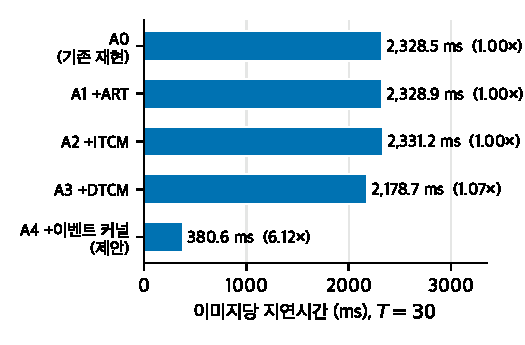
\includegraphics[width=0.92\linewidth]{figures/fig_ablation.pdf}
\caption{누적 절제별 이미지당 지연시간. 페치 계열(A1$\cdot$A2)은
무효과이고, 이득은 데이터 트래픽을 제거하는 이벤트 커널(A4)에
집중된다.}
\label{fig:ablation}
\end{figure}

\subsection{RQ2: 원리별 기여의 분해}\label{sec:rq2}

제안 커널은 한 번에 완성되지 않았다. 원리를 하나씩 실리콘에서
검증하며 다섯 차례 반복했고(그림~\ref{fig:iter}), 이 이력은 원리별
준절제에 해당한다 --- 단 k1에는 원리 2의 요소(2채널 레지스터
블로킹)가 일부 선반영되어 있고, 원리 3의 기여는 속도가 아니라 전
과정 무위반의 정확성 불변식이다. 전 과정에서 출력 체크섬은 한 번도
어긋나지 않았다(P3의 상시 감시).

\textbf{항등식 단독(k1, $2{,}178.7\rightarrow579.2$ms)}: 이벤트
목록을 im2col 컬럼에서 만들고 조밀 레이아웃 가중치를 2채널씩
gather하는 최소 구현만으로 3.8배 --- 식~(\ref{eq:collapse})의 이득이
지배적임이 실증된다. \textbf{P1 완성(k2, $\rightarrow504.3$ms)}:
값 실체화를 제거하고 수용 영역에서 위치를 직접 스캔하자 74.9ms가
추가로 사라졌다 --- im2col 트래픽의 소멸분이다.
\textbf{P2 전반(k3, $\rightarrow457.5$ms)}: 가중치 전치는 예측대로
CPL2를 $249.5\rightarrow148.4$ms로 개선했으나, CPL1은
$228.7\rightarrow282.8$ms로 \textbf{퇴행}했다. CPL1 가중치는 이미
DTCM 상주라 지역성 개선의 여지가 없는데, 이 버전이 누산기를 메모리
배열에 두어 원소당 적재-가산-저장이 추가된 탓이다.
\textbf{P2 후반(k4, $\rightarrow382.2$ms)}: 8채널 레지스터 블로킹이
퇴행을 회복시키며(CPL1 $223.2$ms) CPL2도 추가
개선($132.9$ms)했다. 지역성과 레지스터 상주가 \emph{함께여야}
원리가 성립함을 퇴행-회복 쌍이 보여준다. \textbf{P1의 밀도
적응(k5, $\rightarrow380.6$ms)}: 고밀도 레이어의 무분기 스캔은
1.0ms 개선에 그쳤다 --- 컴파일러가 이미 조건부 실행을 생성하고
있었던 것으로 보이며, 기각된 가설로 기록한다. 측정 출처를
명확히 하면, k1--k4는 하네스 정비(III장) \emph{전}의 개발
기록이고(정비로 제거된 노이즈는 0.2\% 미만) 표~\ref{tab:ablation}의
A계열과 k5는 정비 후 재측정값이다.

\begin{figure}[htbp]
\centering
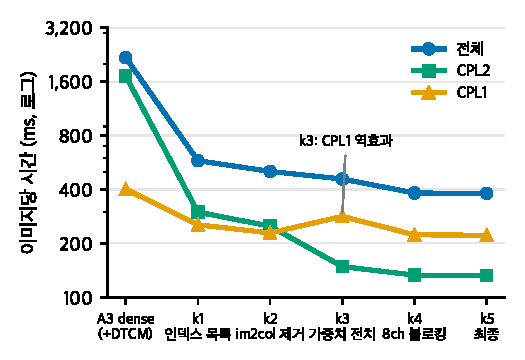
\includegraphics[width=0.95\linewidth]{figures/fig_kernel_iter.pdf}
\caption{원리별 검증의 이력(로그 축). k3의 CPL1 퇴행과 k4의 회복이
원리 2의 두 요소(지역성$\cdot$레지스터 상주)가 각각 필요함을
보인다.}
\label{fig:iter}
\end{figure}

\subsection{RQ3: 레이어 비대칭과 비용 모델}\label{sec:rq3}

그림~\ref{fig:layers}의 레이어 분해가 보이듯, 같은 커널의 이득은
발화 밀도에 따라 크게 갈린다: 밀도 4.1\%의 CPL2는
$1{,}719.8\rightarrow132.2$ms(13.0배), 밀도 47.7\%의 CPL1은
$401.8\rightarrow222.1$ms(1.8배)다. 시간비로는 각각 0.077과
0.553이고, 식~(\ref{eq:costmodel})에 대입하면 $\alpha\approx0.032$,
$\beta\approx1.09$를 얻는다. 두 점으로 두 파라미터를 정하는 것이므로
이는 검증이 아니라 \emph{분해}다. 모델의 내용은 해석에 있다:
$\beta\approx1.09$는 이벤트 1개의 처리 비용(인덱스 적재$+$8채널
가산)이 조밀 원소 1개의 비용(SMLALD MAC$+$피연산자 적재)과 거의
같다는 뜻이고, 따라서 이득은 거의 전적으로 ``건너뛴 원소 수''에서
나온다. $\alpha\approx0.032$는 스캔$\cdot$에필로그의 고정 몫으로,
이 커널 형상의 이득 상한이 약 $1/\alpha\approx31$배임을 말한다 ---
CPL2의 13.0배는 상한의 42\% 지점이다. 모델의 외삽적 함의는 VI장에서
다룬다.

\begin{figure}[htbp]
\centering
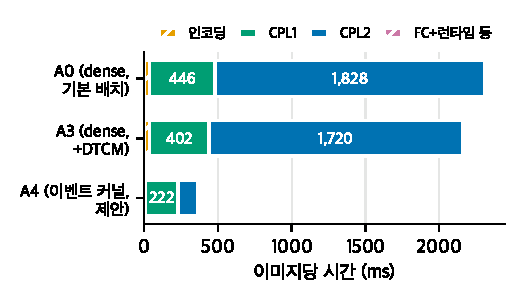
\includegraphics[width=0.95\linewidth]{figures/fig_layers.pdf}
\caption{레이어 분해. 동일 커널의 이득이 발화 밀도에 따라
13.0$\times$(CPL2, 4.1\%)와 1.8$\times$(CPL1, 47.7\%)로 갈린다 ---
병목이 CPL2에서 CPL1로 이동한다.}
\label{fig:layers}
\end{figure}

\subsection{RQ4: 표준 런타임의 대가}

동일 최적화를 적용한 비TFLM 직접 경로 A4$'$는 372.8ms로, 런타임의
대가는 이미지당 7.8ms(2.1\%)다. $T{=}30$회의 Invoke 반복에도
해석기 기반 런타임이 수용 가능한 비용에 머문다는 선행 연구의
결론\cite{cha2026fusion}은 추론이 6배 빨라진 뒤에도 유지된다.
부수적으로, 두 경로는 LIF1 스파이크 진폭이 다름에도(직접 경로
$S_1{=}16{,}384$, TFLM 경로 $32{,}767$ --- 배율은 requantize 계수에
흡수) 출력 체크섬까지 일치했다 --- 계약(4.1절)이 구현 변형에
강건함을 보이는 독립 증거다.

\subsection{계약의 검증}\label{sec:checksum}

회귀 판정은 출력 스파이크 체크섬 --- 매 타임스텝 10개 출력 스파이크
값의 부호 없는 16비트 누적 합(8장$\times$30스텝$\times$10출력,
$2{,}400$개 값) --- 으로 한다. LIF는 막전위가 30스텝에 걸쳐 누적되는
상태 기계이므로 네트워크 어디서든 1 LSB의 차이가 발화 타이밍
연쇄로 증폭된다: 체크섬은 단순하지만 민감하다. 실측 결과
\textbf{A0--A4와 A4$'$, 여섯 빌드의 체크섬이 전부
동일}(0x00E9FE2C)했고 8장의 예측도 전부 일치했다(7/8 정답; 표본
8장은 데모 규모로 정확도 지표가 아니다). 한계도 명시한다: 단순
합이라 오류의 상쇄 우연이 이론상 가능하고 검증 범위는
8장$\times$30스텝이 실행한 경로다. 전자는 예측 일치가, 후자는
4.1절의 구성적 논증이 보완하며, dense 경로 자체의 정당성은 선행
연구의 호스트 검증(LIF SIMD $1{,}887$만 조합 전수 비교
포함)\cite{cha2026fusion}이 담보한다.

\subsection{자원 사용}

최종 빌드(A4)의 정적 사용량은 RAM $283{,}072$B(전치 가중치 사본
154KB와 아레나 64KB 설정 포함), Flash $296{,}432$B이다. TCM 사용은
표~\ref{tab:placement}과 같고(DTCM 89\%, ITCM 30\%), LIF
상태$\cdot$스크래치가 아레나 밖으로 나가면서 TFLM 아레나 실사용은
$79{,}764$B에서 $25{,}940$B로 줄었다. 예산은 링크 타임 ASSERT로
강제된다.


\section{논의}\label{sec:discussion}

\subsection{언제 이벤트 커널이 우세한가}\label{sec:when}

식~(\ref{eq:costmodel})에 V장의 적합값($\alpha\approx0.032$,
$\beta\approx1.09$)을 넣으면 조밀 경로와의 손익분기 밀도는
$\rho^{*}=(1-\alpha)/\beta\approx0.89$다
(그림~\ref{fig:costmodel}). 두 레이어로 정한 1차 모델의 외삽이므로
정밀값이 아니라 규모 추정으로 읽어야 하지만
(두 레이어는 $r$$\cdot$채널 수$\cdot$가중치 상주 위치가 다르고,
밀도는 전수 호스트 평균$\cdot$시간비는 보드 8장 표본이다), 함의는
규모 수준에서도 뚜렷하다: \textbf{활성의 약 90\%가 발화하기
전까지는 이벤트 커널이 우세하다}. 학습된 SNN의 은닉층 발화율이 통상 수 퍼센트대임을
고려하면, SNN의 실질 동작 영역 전체가 희소 우세 구간 안에 있다.
역으로 이 모델은 우세의 끝도 알려 준다: 본 파이프라인의 입력층은
rate coding 탓에 밀도 47.7\%로 예외적으로 높고, 그래서 이득이
1.8배에 그치며 최적화 후 병목이 그리로 이동했다
(V장). 밀도를 코딩 수준에서 낮추는 것 --- 예컨대 시간
코딩 --- 이 커널 개선과 직교하는 다음 지렛대라는 뜻이다.

\begin{figure}[htbp]
\centering
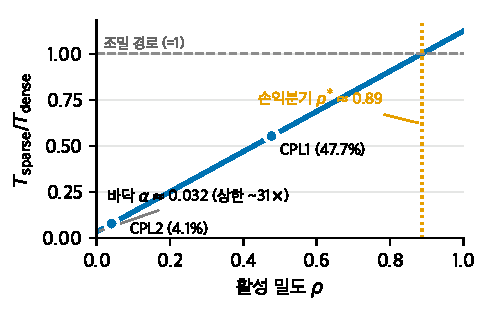
\includegraphics[width=0.9\linewidth]{figures/fig_costmodel.pdf}
\caption{시간비 $T_{\mathrm{sparse}}/T_{\mathrm{dense}}$ 대 활성
밀도 $\rho$. 실측 두 점(CPL1$\cdot$CPL2)으로 정한
식~(\ref{eq:costmodel})의 1차 모델은 손익분기
$\rho^{*}\!\approx\!0.89$와
이득 상한 $1/\alpha\!\approx\!31\times$를 시사한다.}
\label{fig:costmodel}
\end{figure}

\subsection{무엇을 회수했고 무엇이 남는가}

본 연구가 회수한 것은 이벤트 구동성의 \emph{산술적} 몫 --- 0
피연산자의 로드$\cdot$곱셈 제거 --- 이다. 뉴로모픽 하드웨어가
추가로 제공하는 몫, 즉 클럭 없는 비동기 실행$\cdot$이벤트 기반
전력 게이팅$\cdot$메모리-연산 병치는 소프트웨어로 회수되지 않는다.
따라서 본 결과는 뉴로모픽 칩의 대체가 아니라, ``전용 실리콘 없이도
회수 가능한 몫이 정확히 얼마인가''에 대한 한 실측 데이터점이다.
같은 이유로 본 논문은 지연시간을 보고하며, 에너지는 별도 계측
없이 지연 비례 추정 이상을 주장하지 않는다.

방법론 측면에서는 두 가지가 이 결과를 가능하게 했다.
첫째, \emph{의미 보존 계약}(4.1절)이다. 비트 동일성이 상시
검증되는 불변식이었기에 im2col 제거$\cdot$전치$\cdot$블로킹 같은
공격적 재배열을 주저 없이 시도할 수 있었고, k3의 퇴행 같은 실패도
정확성 불안 없이 성능 문제로만 다룰 수 있었다. 둘째, \emph{측정
우선 진단}(III장)이다. 마이크로벤치마크가 지목한 병목을 워크로드
절제로 반증하지 않았다면, 페치 최적화에 노력이 소진되었을 것이다.

\subsection{한계}\label{sec:limits}

본 연구의 한계를 명시한다. (i) 단일 모델$\cdot$단일 보드의
실측이다. 비용 모델이 형상 의존 파라미터를 흡수하지만, 다른
네트워크$\cdot$다른 Cortex-M 등급에서의 $\alpha,\beta$는 재적합이
필요하다. (ii) 체크섬 검증의 범위는 실행된 경로에
국한된다(V장). (iii) 정수 구현의 전체 테스트셋 정확도를 보드에서
직접 실측하지는 못했다 --- 선행 연구와 공유하는 한계다. (iv) 입력층
밀도(47.7\%)는 rate coding의 산물로, 코딩 방식을 바꾸면 이득
분포도 달라진다. (v) 에너지를 직접 계측하지 않았다.


\section{결론}\label{sec:conclusion}

SNN의 효율 약속은 이진 스파이크의 대수에 이미 들어 있다. 본 논문은
그 약속이 범용 MCU 배포 경로의 커널 경계에서 소멸한다는 것, 그리고
하드웨어 변경 없이 --- 세 가지 설계 원리(위치의 실체화, 불규칙
축의 인덱스화, 에필로그 불변)와 의미 보존 계약만으로 --- 비트
단위 동일하게 회수된다는 것을 STM32F746 실측으로 보였다. 결과는
종단 $6.12$배($2{,}328.5\rightarrow380.6$ms/이미지), 발화율 4.1\%
레이어의 동일 배치 dense 대비 13.0배이며, 여섯 빌드 변형의 출력
체크섬 일치가 정확성
주장을 실리콘에서 뒷받침한다. 표준 TinyML 스택은 그대로 남는다:
커스텀 연산자 등록만으로 통합되고 런타임 대가는 2.1\%다. 아울러 통념적
병목(명령 페치)에 대한 두 최적화가 실워크로드에서 무효과였다는
부정적 결과와 그 기제를 함께 보고했다 --- 병목의 위치는
마이크로벤치마크가 아니라 대상 워크로드 위의 절제 실측으로
확정되어야 한다.

향후 과제는 세 방향이다. 첫째, 최적화 후 병목이 된 고밀도
입력층이다: 인코더가 이벤트 목록을 직접 방출하게 하여 수용 영역
재스캔을 제거하는 것은 본 설계의 자연스러운 연장이고, 시간 코딩으로
입력 밀도 자체를 낮추는 것은 커널과 직교하는 지렛대다. 둘째, 비용
모델의 일반화다: 형상$\cdot$밀도가 다른 모델군과 다른 Cortex-M
등급에서 $\alpha,\beta$를 체계적으로 측정하면, 주어진 SNN에 대해
이벤트 커널의 채택 여부를 배포 전에 판정하는 도구가 된다. 셋째,
에너지 직접 계측과 정수 구현의 전 테스트셋 보드 정확도 실측으로
검증의 외연을 넓히는 것이다.


\bibliographystyle{ieeetr}
{\footnotesize
\bibliography{references}
}

\end{document}
